\documentclass{article}
\usepackage{graphicx} % new way of doing eps files
\usepackage{listings} % nice code layout
\usepackage[usenames]{color} % color
\usepackage{float}
\definecolor{listinggray}{gray}{0.9}
\definecolor{graphgray}{gray}{0.7}
\definecolor{ans}{rgb}{1,0,0}
\definecolor{blue}{rgb}{0,0,1}
% \Verilog{title}{label}{file}
\newcommand{\Verilog}[3]{
  \lstset{language=Verilog}
  \lstset{backgroundcolor=\color{listinggray},rulecolor=\color{blue}}
  \lstset{linewidth=\textwidth}
  \lstset{commentstyle=\textit, stringstyle=\upshape,showspaces=false}
  \lstset{frame=tb}
  \lstinputlisting[caption={#1},label={#2}]{#3}
}


\author{your names}
\title{Lab title}

\begin{document}
\maketitle

\section{Executive Summary}
The Executive Summary section should be a single concise paragraph that describes the following items.  Please note that this should be a paragraph, not an itemized list like I have below.  The list is just to tell you what I'm looking for...it is not there for you to fill it in on your lab report.  See the Lab 1 Example Report.pdf on Canvas to see a good example of what I'm looking for.
\begin{enumerate}
	\item The goal of the lab
	\item What modules you created and what they do.  This should describe how the modules function and how they fit into the overall processor that we are building.  For instance, for Lab 1, you will want to describe the operation of the register and the fact that it is used to store the program counter, which is used to keep track of which instruction to execute next.
	\item Whether your lab was successful.  If not successful, please state what is not currently working.
\end{enumerate}	

\section{Test Report}
To verify operation of this/these module(s), this lab requires N test bench(es).  (You can just copy this statement and fill it in with the correct number of test benches)
\begin{enumerate}
	\item Register Test Bench
\end{enumerate}

% This section should display the Expected Results Table and the Simulation Results for each test bench.  Make sure to label each figure correctly.  Please put them in the order of ERT1, SimResults1, ERT2, SimResults2 so that I can easily compare the ERT and Simulation Results.  To force the figures to be positioned correctly, add the float package (at the top of this file) and use the [H] after {figure} as I did below.  Also, if the ERT is on one page and the Simulation Results are on the next page, you can use a pagebreak as I did below so that the ERT goes to the next page also.

\pagebreak

\begin{figure}[H]
	\begin{center}
		\caption{Expected Results of the register test.}\label{fig:ert_registertest}
		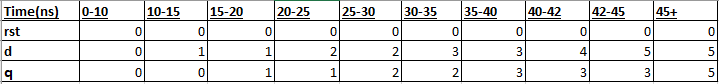
\includegraphics[width=1.0\textwidth]{../images/ert_register_test.png}
	\end{center}
\end{figure}

\begin{figure}[H]
	\begin{center}
		\caption{Timing diagram for the register test.}\label{fig:registertest}
		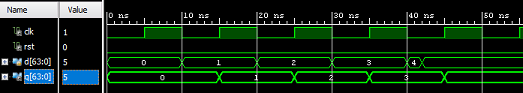
\includegraphics[width=1.0\textwidth]{../images/register_test_timing_diagram.png}
	\end{center}
\end{figure}


\section{Code Appendix}
% The code appendix should include the test bench code and module code for this lab.
\Verilog{Verilog code for testing a register.}{code:regtest}{../code/1_fetch/register_test.v}
\Verilog{Verilog code for implementing a register.}{code:reg}{../code/1_fetch/register.v}
\end{document} 